\section{Visual Servoing in Robotic Manipulation}
Visual servoing is a robotic control technique that utilizes information from a vision sensor to regulate the pose (position and orientation) of a robot's end-effector relative to a target or environmental features \cite{Hutchinson1996}.  It represents the fusion of results from multiple disciplines, including high-speed image processing, kinematics, dynamics, and real-time computing. The fundamental objective is to create a closed-loop control system where visual information is used to minimize a vision-based error signal.

\subsection{Camera Projection Models}
Understanding the geometric mapping of 3D points onto a 2D image plane is fundamental to visual control. This project utilizes two primary models: the standard pinhole model and the fisheye model.

\subsection{The Pinhole Camera Model}
The Pinhole model serves as the ideal geometric basis for most visual servoing control laws. As illustrated in Equation~\ref{fig:pinhole_model}, a 3D point $P = [X, Y, Z]^T$ in the camera frame $\{C\}$ is projected onto the image plane at coordinates $p = [x, y]^T$ via the focal length $\lambda$\cite{Hutchinson1996}:
\begin{equation}
    x = \lambda \frac{X}{Z}, \quad y = \lambda \frac{Y}{Z}
\end{equation}
This linear relationship forms the basis for the \textbf{Interaction Matrix} (Image Jacobian), which relates the velocity of image features to the spatial velocity of the camera.
\begin{figure}[H]
    \centering
    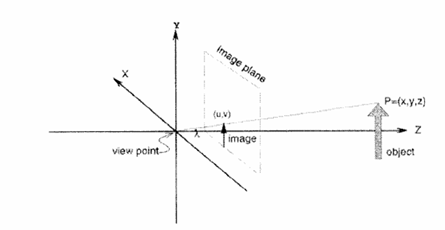
\includegraphics[width=0.5\textwidth]{Figures/chapter2/Visual_servo/pinhole_model.png}
    \caption{Pinhole camera projection model illustrating the mapping of a 3D point $P$ onto the image plane at point $p$ through focal length $\lambda$}
    \label{fig:pinhole_model}
\end{figure}

\subsubsection{The Fisheye Camera Model}
To address the wide Field of View (FoV) requirements of the robotic system—often exceeding $180^{\circ}$ for surround-view perception—a fisheye projection model is employed. Unlike the rectilinear projection of the pinhole model, fisheye lenses utilize non-linear mapping to project a hemispherical field onto a 2D plane.

As described by Cho et al. \cite{Cho2023}, this thesis adopts the \textbf{equidistance projection model} (or $f\text{-}\theta$ model), which approximates the radial distance $\rho$ as directly proportional to the incident angle $\theta$:

\begin{equation}
    \rho_{fisheye} = f \theta
    \label{eq:fisheye_model}
\end{equation}

This contrasts with the standard pinhole model ($\rho = f \tan \theta$), which breaks down as $\theta$ approaches $90^{\circ}$ because the projection distance diverges to infinity. The equidistance model allows the representation of incident rays from very wide angles without this singularity.

\begin{figure}[H]
    \centering
    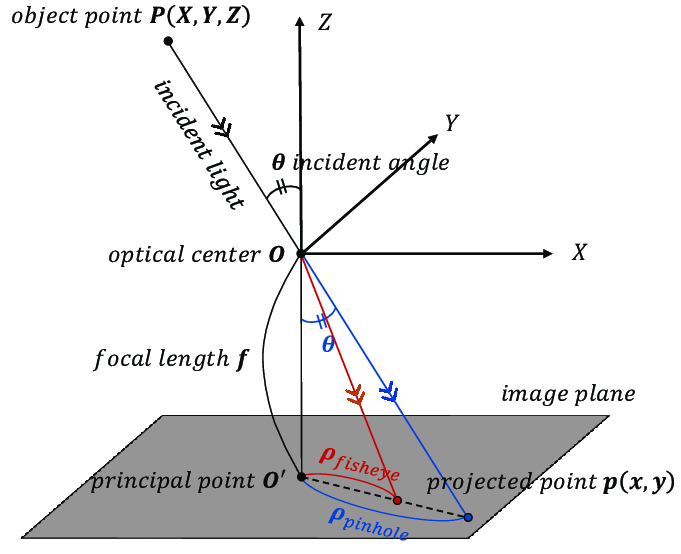
\includegraphics[width=0.6\textwidth]{Figures/chapter2/Visual_servo/fisheye_vs_pinhole.png}
    \caption{Comparison of fisheye equidistance projection (red) and pinhole projection (blue). The fisheye model maintains a linear relationship between incident angle $\theta$ and radial distance $\rho = f\theta$, while the pinhole model uses $\rho = f\tan\theta$, which diverges as $\theta \to 90^{\circ}$.}
    \label{fig:fisheye_vs_pinhole}
\end{figure}

\paragraph{Rectification Strategy}
While fisheye lenses provide a comprehensive field of view, the non-linear distortion creates significant challenges for standard visual servoing algorithms that assume linear projection. However, as noted in the literature, this distortion is \textbf{spatially variant}—the degree of distortion increases significantly towards the image periphery but remains minimal near the optical center \cite{Cho2023}.

Since the manipulation tasks in this project are constrained to the central workspace of the robot (the ``safe region'' of the lens), we employ a \textbf{rectification strategy} (or ``virtual pinhole'' approach). The raw fisheye images are mathematically undistorted to a planar view using camera calibration parameters: the intrinsics matrix $K$ and distortion coefficients $\mathbf{D}$.

The camera intrinsics matrix $K$ encodes the internal optical parameters:
\begin{equation}
    K = \begin{bmatrix} f_x & 0 & c_x \\ 0 & f_y & c_y \\ 0 & 0 & 1 \end{bmatrix}
\end{equation}
where $f_x$ and $f_y$ are the focal lengths (in pixels) in the horizontal and vertical directions, and $(c_x, c_y)$ is the principal point (optical center projection on the image plane). These parameters are obtained through calibration and remain constant for a given camera.

The distortion coefficients $\mathbf{D} = [k_1, k_2, k_3, k_4]^T$ model the fisheye distortion using the equidistance model:
\begin{equation}
    \rho_{distorted} = \left(k_1 \theta + k_2 \theta^3 + k_3 \theta^5 + k_4 \theta^7\right)
\end{equation}
where $\theta$ is the incident angle and the coefficients $k_i$ capture radial distortion at increasing polynomial orders. The undistortion process inverts this relationship to recover the true geometric coordinates.

As validated by Kita et al. \cite{Kita2011} for robotic manipulation tasks, projecting fisheye data onto a specific reference plane significantly reduces shape ambiguity for close-range objects. This process maps the curved fisheye projection back to a linear grid:

\begin{equation}
    p_{rect} = \text{undistort}(p_{fisheye}, K, \mathbf{D})
\end{equation}

This effective linearization allows for the use of standard Interaction Matrices (Jacobians) derived for pinhole cameras. While this method inherently reduces the effective FoV at the periphery \cite{Khomutenko2016}, it maintains high geometric fidelity in the central workspace where grasping operations occur, thereby reducing the computational complexity of the control law without compromising task accuracy.

\subsection{Visual Feature Extraction}
Before control laws can be applied, relevant information must be extracted from the raw image stream. Visual features $s$ serve as the inputs to the control loop and can be classified into geometric primitives (points, lines) or image moments (centroids, areas) \cite{Chaumette2006}.

For robotic grasping applications where the target object is clearly segmented from the background and exhibits a regular geometric shape (e.g., rectangular bricks), \textbf{corner-based features} extracted from the object's bounding geometry are particularly effective. Rather than relying on a single centroid point, the four corners of a bounding rectangle provide redundancy and sufficient constraints for robust pose estimation and visual servoing. These corner points serve as the primary feature vector:

\begin{equation}
    s = [x_{1}, y_{1}, x_{2}, y_{2}, x_{3}, y_{3}, x_{4}, y_{4}]^T
\end{equation}

where each $(x_i, y_i)$ represents the pixel coordinates of corner $i$ in the image plane. This representation provides multiple observables from a single object, improving robustness compared to single-point features while maintaining computational efficiency \cite{Chaumette2006}.

Auxiliary to corner-based features, the object's \textbf{centroid} (computed via image moments) is useful for target disambiguation and stability monitoring. The centroid position and area changes serve as indicators for motion prediction and anomaly detection, though they are not directly used as servoing features.

\subsubsection{Feature Detection Methods in Visual Servoing}
The selection of feature extraction method is fundamental to visual servoing performance. Broadly, features can be categorized into two classes: \textbf{geometric features} (points, lines, edges) and \textbf{appearance-based features} (color, texture, moments). 

Geometric feature detectors such as ORB (Oriented FAST and Rotated BRIEF) \cite{Rublee2011} and AKAZE \cite{Alcantarilla2012} provide scale and rotation invariance with improved computational efficiency over older methods. However, these methods may suffer from poor repeatability in highly controlled environments where objects have limited texture or in cluttered scenes where spurious corners are abundant. Conversely, when target objects possess distinct visual properties (e.g., color), appearance-based methods offer computational efficiency and robustness to geometric variations \cite{Chaumette2006}.

\paragraph{Color-Space Segmentation Approaches}
In structured manipulation environments, \textbf{color-space segmentation} provides a practical foundation for feature extraction. Compared to RGB space, which couples luminance and chrominance information, the HSV (Hue, Saturation, Value) color space decouples these components, providing robustness to illumination variations \cite{Fairchild2013}. Thresholding in HSV space isolates pixels belonging to target objects, yielding a binary segmentation mask.

Connected-component analysis identifies distinct spatial clusters (blobs) within the segmented region. For each blob, geometric properties—centroid, area, orientation, and bounding geometry—are computed and used as feature vectors. This approach is computationally efficient and particularly effective in industrial settings where target objects are deliberately assigned distinct colors for reliable identification \cite{Bradski2008}.

\begin{figure}[H]
    \centering
    \includegraphics[width=0.6\textwidth]{Figures/chapter2/Visual_servo/hsv_color_space.png}
    \caption{HSV color space representation showing hue ($H$), saturation ($S$), and value ($V$) components...}
    \label{fig:hsv_color_space}
\end{figure}

\subsection{Control Architectures}
\label{sec:control_architectures}
\subsubsection{Position-Based Visual Servo (PBVS)}
PBVS involves reconstructing the 3D pose of the target with respect to the camera frame \cite{Hutchinson1996}. The error signal is defined in the Cartesian task space ($x, y, z, \text{roll, pitch, yaw}$). While intuitive, PBVS is highly sensitive to camera calibration errors and relies on accurate 3D models of the target object.

\begin{figure}[H]
    \centering
    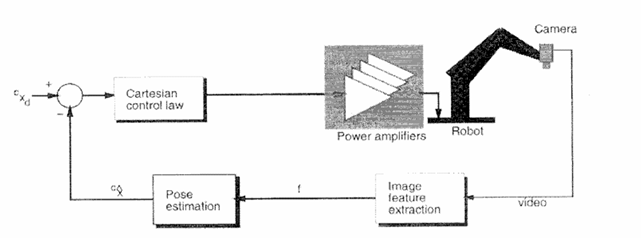
\includegraphics[width=0.6\textwidth]{Figures/chapter2/Visual_servo/pbvs_diagram.png}
    \caption{Position-Based Visual Servo (PBVS) architecture showing the transformation from 3D Cartesian task space to camera frame control.}
    \label{fig:pbvs_diagram}
\end{figure}

\subsubsection{Image-Based Visual Servo (IBVS)}
\label{sec:ibvs_theory}
IBVS defines the control task directly in the 2D image feature space. The error signal is defined as $e(t) = s(t) - s^*$, where $s$ is the current feature vector and $s^*$ is the desired feature vector. The relationship between feature velocity $\dot{s}$ and camera velocity $v_c$ is given by the Interaction Matrix $L_s$ \cite{Chaumette2006}:

\begin{figure}[H]
    \centering
    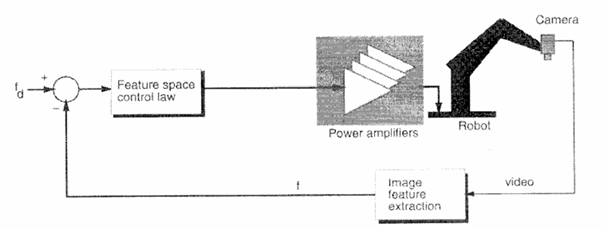
\includegraphics[width=0.6\textwidth]{Figures/chapter2/Visual_servo/ibvs_diagram.png}
    \caption{Image-Based Visual Servo (IBVS) architecture showing error minimization directly in 2D image feature space.}
    \label{fig:ibvs_diagram}
\end{figure}

\begin{equation}
    \dot{s} = L_s v_c
\end{equation}
IBVS is generally more robust to calibration errors than PBVS because it regulates error directly in the image plane.

\paragraph{The Interaction Matrix (Image Jacobian)}
The Interaction Matrix $L_s$, also referred to as the Image Jacobian, is a fundamental component of IBVS that relates the rate of change of image features to the velocity of the camera in 3D space. For a point feature at coordinates $(u, v)$ at depth $Z$ from the camera frame, the Interaction Matrix takes the form \cite{Chaumette2006}:

\begin{equation}
    L_s(u, v, Z) = \begin{bmatrix} -\frac{1}{Z} & 0 & \frac{u}{Z} & uv & -(1+u^2) & v \\ 0 & -\frac{1}{Z} & \frac{v}{Z} & 1+v^2 & -uv & -u \end{bmatrix}
\end{equation}

where the six columns correspond to the six degrees of freedom of camera motion: translational velocities $(v_x, v_y, v_z)$ and rotational velocities $(\omega_x, \omega_y, \omega_z)$. The matrix maps camera velocity $v_c = [v_x, v_y, v_z, \omega_x, \omega_y, \omega_z]^T$ to the feature velocity $\dot{s}$.

The critical dependency on depth $Z$ necessitates depth estimation or availability of a depth sensor for accurate control. For multiple features, the Interaction Matrix is stacked vertically to form a rectangular matrix, providing redundancy and improving robustness to partial occlusions and feature tracking failures.

The control law is derived by inverting the Interaction Matrix:
\begin{equation}
    v_c = -\lambda L_s^+ e = -\lambda L_s^+ (s - s^*)
\end{equation}
where $L_s^+$ is the pseudo-inverse of $L_s$, $\lambda$ is a gain parameter controlling convergence rate, and $e$ is the feature error vector.

\paragraph{Depth Estimation in Monocular IBVS}
A critical challenge in monocular IBVS is that the Interaction Matrix $L_s$ depends on the depth $Z$ of the feature point relative to the camera frame, which is inherently unobservable with a single camera. To address this without external depth sensors, an \textbf{Area-Based Depth Approximation} is employed. By exploiting the projective geometry of planar objects, Chaumette established that the depth $Z$ is inversely proportional to the square root of the object's image area ($A \propto 1/Z^2$) \cite{Chaumette2004}. The estimated depth $\hat{Z}$ can be updated online using the scalar relationship:
\begin{equation}
    \hat{Z} = Z^* \sqrt{\frac{A^*}{A_{current}}}
\end{equation}
where $Z^*$ is the depth at the desired goal position and $A^*$ is the desired feature area. This approximation allows the interaction matrix to be updated dynamically as the robot moves, ensuring the control law remains valid throughout the approach phase \cite{Chaumette2004}.

\subsection{Homography-Based Estimation and Transfer}
To bridge the gap between global perception (fixed camera) and local manipulation (eye-in-hand), \textbf{Homography-based methods} are used for both reconstruction and feature transfer.

\begin{figure}[H]
    \centering
    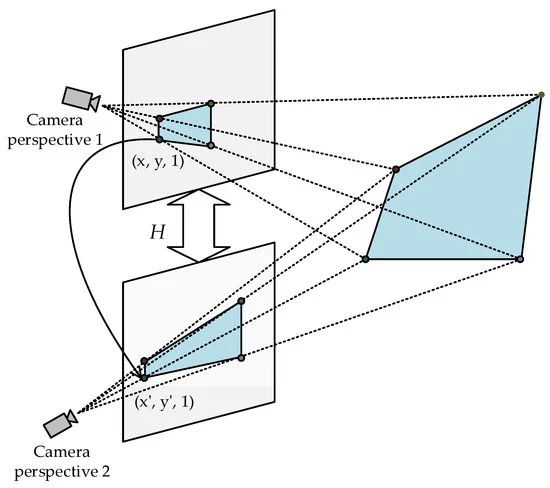
\includegraphics[width=0.7\textwidth]{Figures/chapter2/Visual_servo/homography_geometry.png}
    \caption{Planar homography transformation relationship between two camera perspectives, showing the projection of a planar target through homography matrix $H$.}
    \label{fig:homography_geometry}
\end{figure}

A homography matrix $H$ describes the projective mapping between two images of the same planar surface \cite{Fang2002}. In a multi-camera setup, $H$ relates the pixel coordinates of a target in the global view ($m_{global}$) directly to the corresponding coordinates in the local eye-in-hand view ($m_{local}$):
\begin{equation}
    m_{local} = H m_{global}
\end{equation}

This \textbf{Feature Transfer} capability is crucial for "Global-to-Local Handoff" strategies. It allows the system to identify a grasp point in a high-resolution global camera and mathematically transfer that target point into the local camera's frame, initializing the visual servoing loop without requiring the local camera to perform a wide-area search.

Additionally, for pose estimation, the homography matrix $H$ can be decomposed into the rotation $R$, translation $t$, and plane normal $n^*$ relating the two camera views:
\begin{equation}
    H = R + \frac{t}{d^*}n^{*T}
\end{equation}
This decomposition enables a "Look-and-Move" strategy, allowing the robot to estimate its relative pose to a target for initial open-loop alignment before switching to closed-loop visual servoing.